
% Eigener Beitrag: Beschreibung, Begründung, Aufzeigung, Methode, Fazit

\chapter{Social Engineering}
\label{sec:socialengineering}

\section{Begriffserklärung}
\label{sec:socialengineering:begriffserklaerung}
Zur Erklärung des Begriffs des Social Engineering zeigt man am besten Beispiele auf:

\begin{quote}
	Hallo! Ich bin neu hier, wie komme ich nochmal ins Wifi? \footcite{Social_Engineering_Wenn_die_Gefahr_im_Anzug_kommt__t3n_2015-04-26}
\end{quote}

So einfach kann ein Angriff durch ein Social Engineer aussehen. In dem Beispiel wird versucht sich eine Dienstleistung zu erschleichen. Es gibt keine "`Hacks"' im eigentlichen Sinne. Niemand hängt sich ins Wireless rein, analysiert den Datenverkehr und versucht das Passwort zu knacken.

Angriffe können auch komplexer sein. Man stelle sich ein Unternehmen in Zürich vor, in welches Lastwagen einfahren. Oft haben Lastwagenfahrer ihren Namen auf einem Schild an der Frontscheibe aufgeschrieben. Sobald sich das Tor öffnet und der LKW einfährt, kann man dem Lastwagen nachrennen und den Namen des Fahrers rufen. So kommt man an den Sicherheitsbeamten am Tor vorbei. 
Der Angreifer möchte nun in die Abteilung Forschung \& Entwicklung. Er fragt eine Mitarbeiterin nach dem Weg, mit der Begründung, dass er von einer Tochterfirma in Basel kommt und die Wegbeschreibung am Empfang wohl falsch verstanden hätte. Die Mitarbeiterin gibt bereitwillig Auskunft.
Beim Gebäude der Abteilung Forschung \& Entwicklung ist die Türe abgeschlossen. Nun wartet der Angreifer mit Sicht auf die Türe, bis ein Mitarbeiter dort eintritt. Mit diesem zusammen betritt er das Gebäude. 
Der Angriff lässt sich nun beliebig weiterführen. Vielleicht hängt irgendwo eine Liste mit Telefonnummern oder ein Mitarbeiter hat Notizen an seinem Bildschirm angeklebt mit welchen der Angreifer weiterarbeiten kann. \footcite{Beispiel_fr_einen_Social_Engineering_Angriff_Social_Engineering_-_Manipulation_2015-04-26}

Dieser Angriff nutzt verschiedene Schwachstellen aus. Allen gemein ist dass sie nichts direkt mit Informatik zu tun haben und deshalb in der Kategorie des Social Engineering anzusiedeln sind. Dies wäre der Name an der Windschutzscheibe des LKW's, die Hilfsbereitschaft der Mitarbeiter oder dass offenhalten einer abgeschlossenen Türe für einen Kollegen.

Social Engineering muss nicht immer krimineller Natur sein. das nächste Kapitel setzt sich mit dieser Thematik auseinander.

\section{Typen von Social Engineers}
Social Engineering kann verschiedene Formen annehmen. Diese können bös- oder gutwillig sein. Folgend eine nicht abschliessende Liste von Aktivitäten\footcite{human_hacking} welche mit Social Engineering in Bezug gebracht werden kann:

\begin{itemize}
\item Hacker
\item Spione
\item Identitätsdiebe
\item Verärgerte Angestellte
\item Penetrationstester
\item Regierungen
\item Ärzte, Psychologen, Rechtsanwälte
\item Personalvermittler
\item Verkaufspersonal 
\end{itemize}

Gemeinsam haben diese Jobs, dass sie sich mit der Domäne, in welchen sie agieren, auskennen müssen, viele Informationen zu sammeln haben und ein geschickter Umgang mit Kommunikation besitzen müssen.

\textit{Spione} und \textit{Identitätsdiebe} müssen Informationen über das Ziel sammeln, sich in eine Rolle hineinversetzten und auch Kommunizieren wie diese.

\textit{Verärgerte Angestellte} können grossen Schaden anrichten. Mister X wird entlassen. Beim Gespräch mit dem Chef zeigt er sich verständnisvoll. Sobald er am Arbeitsplatz zurückkehrt beginnt er wichtige Daten zu löschen oder gibt diese weiter. Mister X darf sich nichts anmerken lassen. Muss Kommunizieren wie er es immer tut und den anderen Mitarbeitern etwas vortäuschen.
\textit{Penetrationstester} untersuchen Software auf Fehler. Dabei müssen sie sich in die Lage eines Hackers versetzen, so denken und handeln, wie dieser es tut. Dies umfasst deshalb die gleichen Kompetenzen eines Hackers.

\textit{Regierungen}, \textit{Ärzte}, \textit{Psychologen} und \textit{Rechtsanwälte} haben eines gemeinsam haben. Eine gute Kommunikation. Wie verkaufe ich etwas? Wie vermittle ich dem Volk etwas damit es nicht falsch verstanden wird? Wie überbringe ich eine schlechte Botschaft möglichst sanft? All diese Fragen bedienen sich dem Arsenal des Social Engineerings.

\textit{Personalvermittler} und \textit{Verkaufspersonal} müssen über ihre Produkte und die Kunden wichtige Informationen besitzen, sowie gutes Verhandlungsgeschick besitzen.

Es wurde an Beispielen gezeigt, dass Informationen sammeln und eine geschickte Kommunikation zwei Schlüsselaspekten des Social Engineerings darstellen. Das erste Thema welches nun genauer betrachtet wird ist das Sammeln von Informationen.

\section{Informationssammlung}
Informationen sind das Fundament des Social Engineering. Ist die Basis schief, kann man keine geschickte Angriffe durchführen. Die Aufgabe der Informationssammlung gliedert sich dabei in zwei Bereiche. Die Beschaffung und die Organisation der Daten. Jede erdenkliche Quelle von Informationen sollte dabei durchsucht werden. Ein Haufen von undurchsuchbaren Daten nützt jedoch dem besten Social Engineer nichts. Deshalb müssen diese geordnet und durchsuchbar gegliedert werden.

\subsection{Quellen}
Ein Social Engineer ist nicht wählerisch in der Auswahl seiner Informationsquellen. Webseiten, Blogs, Suchmaschinen, Whois-Abfragen, Öffentliche Server, Social Media und öffentliche Berichte ist eine nicht abschliessende Liste von verlässlichen Datenquellen. 

Man muss sich jedoch nicht nur auf online Medien beschränken. Durch Observation von Personen, Fahrzeugen oder Gebäuden können wertvolle Informationen gewonnen werden. Zu guter letzt darf sich ein Social Engineer auch nicht zu schade sein Abfälle zu durchwühlen. Diese Aktivität wird auch liebevoll Dumpster-Diving oder Garbage-Picking genannt. 

Es ist verblüffend, wie viele Wertvolle Informationen im Müll landen. Checks, Gehaltslisten, Telefonnummern, Namen oder sogar Passwörter werden oft im Abfall entsorgt. Auch wenn sich die Opfer mühe geben und die Unterlagen zuerst durch einen Dokumentenschredder unkenntlich machen nützt dies nichts. Nach ein paar Stunden kann man die Streifen zu einem ganzen Papier zusammenfügen. 

\begin{figure}[htb]
  \begin{subfigure}[b]{.45\linewidth}
    \centering
    
\includegraphics[width=0.5\linewidth]{images/shredded-paper.jpg}
    \caption{Geschreddertes Dokument}
    \label{fig:socialengineering:informationssammlung:quellen:schreddern:subfigures:a}
  \end{subfigure}%
  \begin{subfigure}[b]{.45\linewidth}
    \centering
    
\includegraphics[width=0.5\linewidth]{images/reassembled-shredded-paper.jpg}
    \caption{Zusammengesetztes Dokument}
    \label{fig:socialengineering:informationssammlung:quellen:schreddern:subfigures:b}
  \end{subfigure}
  \caption{Schreddern eines Dokumentes}
  \label{fig:socialengineering:informationssammlung:quellen:schreddern:figures}
\end{figure}

Das einzig verlässliche ist ein Zwei-Wege-Schredder. Solch unkenntlich gemachte Informationen lassen sich nicht mehr zusammenfügen.

\begin{figure}[H]
  \centering
  
\includegraphics[width=0.4\textwidth]{images/two-way-shredded-paper.jpg}
  \caption[Test image for television]{Zwei-Wege geschreddertes Dokument}
  \label{fig:socialengineering:informationssammlung:quellen:zwei-wege-schreddern}
\end{figure}

\subsection{Datenorganisation}
Beim der Sammlung können schnell ein paar Hundert Megabytes an Daten angehäuft werden. Dann stellt sich die Frage wie diese in eine ordentliche Form gebracht werden können. 

Hier gibt es Tool die einen Social Engineer in seiner Sammelwut unterstützen. Wichtige Aspekte einer solchen Software ist es, dass sie einfach zu bedienen und übersichtlich ist. Denn man wird viel Zeit mit ihr verbringen. Natürlich muss sie auch mit grossen Datenmengen umgehen können und jegliche Formen von Daten unterstützen. Dies geht über Text, Bildern bis zu PDF und weiteren Dateien. 

Ein einfaches Tool stellt BasKet dar. Es ist ein OpenSource Tool welches unter der GNU GPL v2 Lizenz betrieben wird und läuft mit Windows, Mac und Linux. Wie der Name bereits aussagt ist es ein Korb für die Ablage von jeglichen Daten.

\begin{figure}[htb]
  \centering
  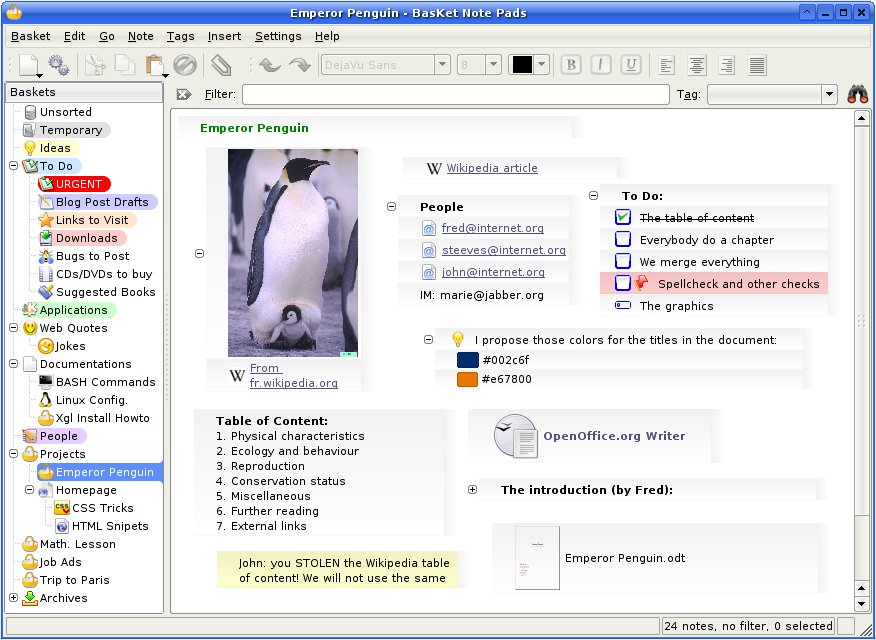
\includegraphics[width=0.8\textwidth]{images/basket.png}
  \caption[Test image for television]{BasKet ermöglicht die einfache Ablage von jeglichen Informationen}
  \label{fig:socialengineering:informationssammlung:datenorganisation:basket}
\end{figure}

Wenn man in einem Team arbeitet, muss eine gemeinsame Ablage der Daten möglich sein. Hier schafft das Programm Dradis abhilfe. Es läuft unter der gleichen Opensource Lizenz wie BasKet und ist auch für die selben Betriebsysteme verfügbar. 

Bei Dradis handelt es sich um ein Webapplikation. Das ganze Team kann dabei auf einer Webseite kollaborieren.

\begin{figure}[htb]
  \centering
  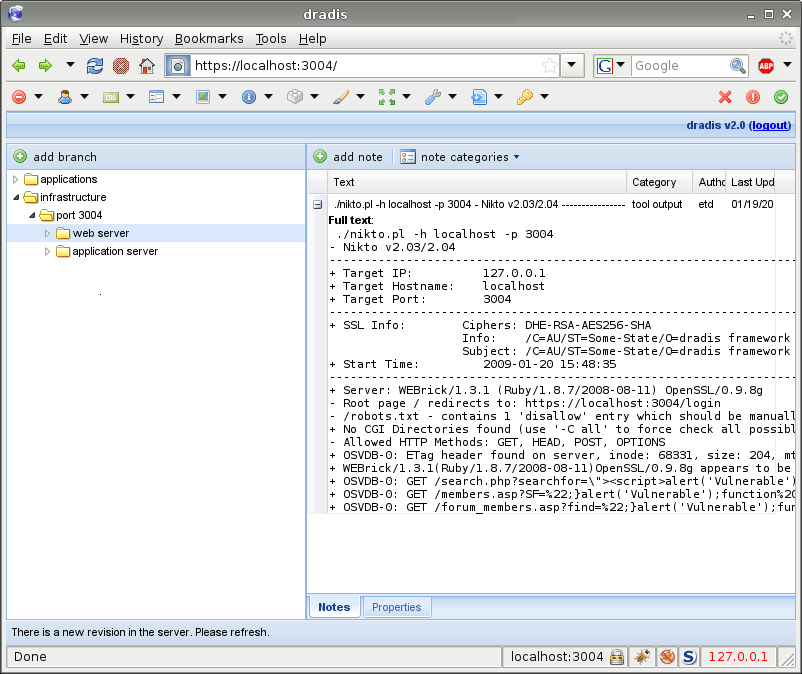
\includegraphics[width=0.8\textwidth]{images/dradis.png}
  \caption[Test image for television]{Mit Dradis können Teams zusammen arbeiten}
  \label{fig:socialengineering:informationssammlung:datenorganisation:basket}
\end{figure}

\section{Kommunikation}
Kommunikation ist eine wichtige Waffe für einen Social Engineer.